\documentclass[a4paper,11pt]{beamer}
\usepackage{etex}
\usepackage{lmodern}
\usepackage[french]{babel}
\usepackage[T1]{fontenc}
\usepackage[utf8]{inputenc}
% \usepackage{listings}
\usepackage{graphicx} 
\usepackage{ragged2e}
\usepackage{enumitem}
\usepackage{array}
% \usepackage{tikz} 
% \usepackage{pgf-umlcd} 
\usepackage{csquotes}
\usepackage{pst-sigsys}
\usepackage{amsmath,amsfonts,bm}
\usepackage{pstricks-add}
% \usepackage{physics}
% \usepackage{ulem}
% \usepackage{wasysym}
\usepackage{hyperref}
\usepackage{matlab-prettifier} 
% \usepackage[dvipsnames]{xcolor}
\usepackage{bm}

\setenumerate{label*=\arabic*.} 

\setbeamertemplate{navigation symbols}{}  
  
\usetheme{Darmstadt} 
\setbeamertemplate{footline}{\insertframenumber/\inserttotalframenumber}
\title{L3 - CMI017 : Signaux et Systèmes\\Séquence V}
\author{BULOUP Frank}
\institute{Aix Marseille Université\\Institut des Sciences du Mouvement}
\date{}

\setbeamertemplate{footline} 
{  
	\begin{beamercolorbox}[ht=2.5ex,dp=1.125ex,%
      leftskip=.3cm,rightskip=.3cm plus1fil]{title in head/foot}%
      {\usebeamerfont{title in head/foot}\insertshorttitle} \hfill    
      \insertframenumber / \inserttotalframenumber%
    \end{beamercolorbox}%
%     \begin{beamercolorbox}[colsep=1.5pt]{lower separation line foot}
%     \end{beamercolorbox} 
}

\newcounter{exampleBlockCounter}
\setcounter{exampleBlockCounter}{1}

\definecolor{comment}{rgb}{0.12, 0.38, 0.18 } %adjusted, in Eclipse: {0.25, 0.42, 0.30 } = #3F6A4D
\definecolor{keyword}{rgb}{0.37, 0.08, 0.25}  % #5F1441
\definecolor{string}{rgb}{0.06, 0.10, 0.98} % #101AF9
\definecolor{myGreen}{rgb}{0,0.4,0}

% \lstset {language=Java,
%  frame=single,
%  frameround=tttt,
%  rulesepcolor=\color{black},
%  showspaces=false,showtabs=false,tabsize=2,
%  numberstyle=\tiny,numbers=left,
%  stringstyle=\color{string},
%  keywordstyle = \color{keyword}\bfseries,
%  commentstyle=\color{comment}\itshape,
%  basicstyle=\ttfamily\footnotesize,
%  breaklines=true,
%  captionpos=b
% }

% \renewenvironment{package}[2][\umlcdPackageTitle]{
% \edef\umlcdPackageTitle{#2}
% \def\umlcdPackageFit{}
% \def\umlcdPackageName{#1}
% }{
%   \begin{pgfonlayer}{background}
%   \node[umlcd style, draw, inner sep=0.5cm, fit = \umlcdPackageFit] (\umlcdPackageName) {};
%   \node[umlcd style, draw, outer ysep=-0.5, anchor=south west] (\umlcdPackageName caption) at
%   (\umlcdPackageName.north west) {\umlcdPackageTitle};
%   \end{pgfonlayer}
% }

\begin{document}

\begin{frame}[plain]  
	\titlepage  
	\center{\includegraphics[scale=0.75]{images/by-nc-sa.eps}}
	\vspace{1cm}
	
	\includegraphics[scale=0.6]{images/LogoAMU.png}\hspace*{2cm}
	\includegraphics[scale=0.2]{images/LogoCNRS.eps}\hspace*{2cm}
	\includegraphics[scale=0.1]{images/LogoISM.eps}
\end{frame} 
  

\begin{frame}{Plan de cette séquence}
	\tableofcontents[hideallsubsections]
\end{frame}

\AtBeginSection[]{
\begin{frame}{Signaux et Systèmes}
	\tableofcontents[currentsection,hideallsubsections]
\end{frame}
}

\begin{frame}{Rappels 1/3}
\begin{alertblock}{Rappel I}
\justifying
Un phénomène périodique élémentaire peut être caractérisé par une cosinusoïde
d'amplitude, de phase et de fréquence spécifiques.
\end{alertblock}
\pause
\begin{alertblock}{Rappel II}
\justifying
Pratiquement tous les signaux périodiques peuvent être développés en série de
Fourier. C.a.d. en combinaison linéaire de phénomènes périodiques élémentaires.
Chacun de ces phénomènes étant caractérisés par le triplet [Amplitude, Phase,
Fréquence]
\end{alertblock}
\pause
\begin{alertblock}{Rappel III}
\justifying
On peut représenter ces triplets de manière graphique sous la forme des spectres
d'amplitude et de phase monolatéraux et bilatéraux.
\end{alertblock}
\end{frame}

\begin{frame}{Rappels 2/3}
\begin{alertblock}{Rappel IV}
\justifying
Cette représentation permet de considérer les signaux d'un point de vue
« fréquentiel » : à quelles fréquences le signal comporte-t-il de l'energie ?
\end{alertblock}
\pause
\begin{alertblock}{Rappel V}
\justifying
La version numérique de l'analyse de Fourier est appelée Transformée de
Fourier Discrète. Il existe un algorithme optimisé nommé Transformée de
Fourier Rapide (Fast Fourier Transform). La fonction Matlab \textbf{fft} permet
de réaliser ce calcul.
\end{alertblock}
\end{frame}

\begin{frame}{Rappels 3/3}
\begin{alertblock}{Rappel VI}
\justifying
On peut obtenir la réponse d'un SDLIT à n'importe quelle entrée en utilisant la
relation de convolution entrée/réponse impulsionnelle :
$$
s(n) = \sum_{k=0}^{+\infty} e(k)h(n-k)
$$
Que l'on peut réécrire de cette façon :
$$
s(n) = \sum_{k=0}^{+\infty} h(k)e(n-k)
$$
Cf. démo annexée.
\end{alertblock}
\end{frame}

\section{Réponse en fréquence des SDLIT}
\subsection{Réponse d'un SDLIT à une cosinusoïde}
 
\begin{frame}
\begin{exampleblock}{?` Question ?}
\justifying
Quelle est la réponse d'un SDLIT lorsque son entrée est une cosinusoïde ?
On notera $\mathcal{H}(z)=\rho(z)e^{i\phi (z)}$ sa fonction de transfert en $z$.
\begin{figure}
	\begin{pspicture}[showgrid=false](0,0)(9,2)
		\psset{arrows=->}
		\pssignal(1.5,1){e}{$\begin{cases}
		\text{Signal d'entrée}\\
		cos(2\pi f_0 nT_e)
		\end{cases}$}
		\psfblock[framesize=1.75 1.65](4.5,1){h}{$\mathcal{H}$}
		\ncline{e}{h}
		\pssignal(7.5,1){s}{$\begin{cases}
		\text{Signal de sortie}\\
		?
		\end{cases}$}
		\ncline{h}{s}
	\end{pspicture}
\end{figure}
\end{exampleblock}
\end{frame}

\begin{frame}
\justifying
On peut réécrire l'entrée de la façon suivante :
$$
e(n) = \frac{1}{2}[z_0^n+ \overline{z_0}^n]
$$
Avec :
$$
\begin{cases}
z_0 &= e^{i\Omega_0}\\
\overline{z_0} &= e^{-i\Omega_0}\\
\Omega_0 &= 2\pi \frac{f_0}{f_e}
\end{cases}
$$
\pause
Pour trouver la sortie il faut résoudre l'équation de convolution :
$$
\begin{aligned}
s(n) &= \sum_{k=0}^{+\infty} h(k)e(n-k)\\
\pause
	 &= \frac{1}{2}z_0^n\cdot\textcolor{red}{\sum_{k=0}^{+\infty} h(k)z_0^{-k}} +
	 \frac{1}{2}\overline{z_0}^n\cdot\textcolor{myGreen}{\sum_{k=0}^{+\infty} h(k)\overline{z_0}^{-k}}\\
\pause
	 &= \frac{1}{2}z_0^n \cdot\textcolor{red}{\mathcal{H}(z_0)} + \frac{1}{2}\overline{z_0}^n
	 \cdot\textcolor{myGreen}{\mathcal{H}(\overline{z_0})}
\end{aligned}
$$
\end{frame}

\begin{frame}
\justifying
Comme $h(n)$ est réelle, on a $\mathcal{H}(\overline{z_0}) =
\overline{\mathcal{H}(z_0)}$ et comme
$\overline{z_0}^n=\overline{z_0^n}$, on trouve :
$$
\begin{aligned}
s(n) &= \frac{1}{2}z_0^n \cdot\mathcal{H}(z_0) + \frac{1}{2}\overline{z_0^n
	 \cdot\mathcal{H}(z_0)}\\
	 &= \Re[z_0^n \cdot\mathcal{H}(z_0)]\\
s(n) &= \bm{\textcolor{red}{\rho(z_0)}} cos[\Omega_0 n +
	 \bm{\textcolor{myGreen}{\phi(z_0)}}]
\end{aligned}
$$
\pause
\vspace{0.1cm}

\textbf{
La sortie est donc également une cosinusoïde de même fréquence que l'entrée.
Mais :
\pause
\begin{itemize}[label=$\bullet$]
  \item \textcolor{red}{son amplitude a été pondérée par le module de la
  fonction de transfert du système à cette fréquence} 
  \pause
  \item \textcolor{myGreen}{sa phase  a été augmentée de l'argument de la
	fonction de transfert du système à cette fréquence}. 
\end{itemize}
}
\end{frame}

\begin{frame}
\begin{exampleblock}{?` Question ? $\Rightarrow$ Réponse !}
\justifying
Quelle est la réponse d'un SDLIT lorsque son entrée est une cosinusoïde ?
On notera $\mathcal{H}(z)=\rho(z)e^{i\phi (z)}$ sa fonction de transfert en $z$.
\begin{figure}
	\begin{pspicture}[showgrid=false](0,0)(10.5,2)
		\psset{arrows=->}
		\pssignal(1.5,1){e}{$\begin{cases}
		\text{Signal d'entrée}\\
		cos(2\pi f_0 nT_e)
		\end{cases}$}
		\psfblock[framesize=1.75 1.65](4.5,1){h}{$\mathcal{H}$}
		\ncline{e}{h}
		\pssignal(8.25,1){s}{$\begin{cases}
		\text{Signal de sortie}\\
		s(n)=\\
		\rho(f_0)cos[2\pi f_0 nT_e + \phi(f_0)]
		\end{cases}$}
		\ncline{h}{s}
	\end{pspicture}
\end{figure}
Avec :
\begin{itemize}[label=$\bullet$]
  \item $\rho(f_0)=\left\lvert
  \mathcal{H}\left(e^{i2\pi\frac{f_0}{f_e}}\right) \right\rvert$
  \item $\phi(f_0)=Arg\left[  \mathcal{H}\left(e^{i2\pi\frac{f_0}{f_e}}\right)
  \right]$
\end{itemize}
\end{exampleblock}
\end{frame}

\begin{frame}
\begin{alertblock}{Remarque I}
\justifying
Mais d'après les séries de Fourier, presque tous signal peut être décomposé en
somme de cosinusoïdes. On peut donc représenter l'entrée d'un système comme une
somme de cosinusoïdes. 
\end{alertblock}
\pause
\begin{alertblock}{Remarque II}
\justifying
Comme on ne considère que les SDLIT, la sortie sera
également une composition de cosinusoïdes dont les amplitudes et les phases
seront modifiées par les caractéristiques de la fonction de transfert du système
aux fréquences présentent dans le signal d'entrée.
\end{alertblock}
\end{frame}

\subsection{Illustration}
\begin{frame}
\centering
Signal d'entrée : $e(n) = 2\cdot cos(2\pi 25 nT_e) + 6\cdot cos(2\pi 100 nT_e)$
\vspace{0.25cm}

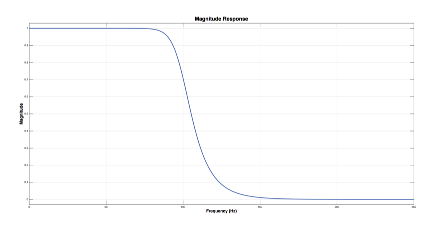
\includegraphics[scale=1.5]{images/MagFilter1_BIS.eps}

\begin{exampleblock}{?`  Question ?}
\centering
Quelles sont les amplitudes des sinusoïdes en sortie du système ?
\end{exampleblock}

\end{frame}

\begin{frame}
\centering
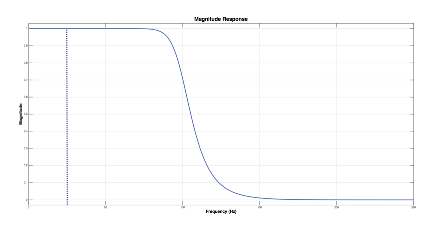
\includegraphics[scale=1.5]{images/MagFilter2_BIS.eps}
\begin{itemize}[label=$\bullet$]
  \item À $25Hz$, le «gain» est de $1$
\end{itemize}
\end{frame}

\begin{frame}
\centering
\includegraphics[scale=1.5]{images/MagFilter3_BIS.eps}
\begin{itemize}[label=$\bullet$]
  \item À $25Hz$, le «gain» est de $1$
  \item À $100Hz$, il est d'environ $0.7$
\end{itemize}
\end{frame}

\begin{frame}
\centering
Signal d'entrée : $e(n) = 2\cdot cos(2\pi 25 nT_e) + 6\cdot cos(2\pi 100 nT_e)$
\vspace{0.25cm}

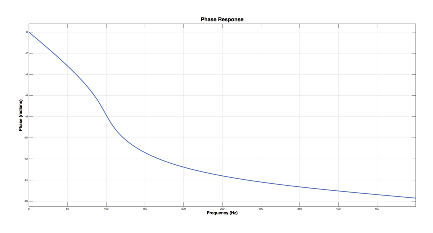
\includegraphics[scale=1.5]{images/PhaseFilter1_BIS.eps}

\begin{exampleblock}{?`  Question ?}
\centering
Quelles sont les «décalages» des phases des sinusoïdes en sortie du système ?
\end{exampleblock}

\end{frame}

\begin{frame}
\centering
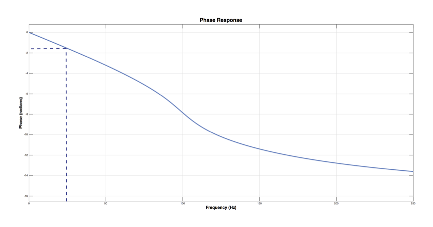
\includegraphics[scale=1.5]{images/PhaseFilter2_BIS.eps}
\begin{itemize}[label=$\bullet$]
  \item À $25Hz$, le «décalage» de phase est d'environ $-1.5rd$
\end{itemize}
\end{frame}

\begin{frame}
\centering
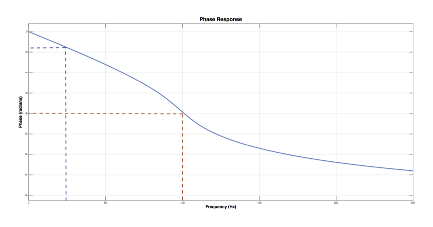
\includegraphics[scale=1.5]{images/PhaseFilter3_BIS.eps}
\begin{itemize}[label=$\bullet$]
  \item À $25Hz$, le «décalage» de phase est d'environ $-1.5rd$
  \item À $100Hz$, il est d'environ $-8rd$
\end{itemize}
\end{frame}

\begin{frame}
\centering
Le signal de sortie du système est donc le suivant :
$$
\begin{aligned}
s(n) &= 1\cdot 2\cdot cos(2\pi 25 nT_e - 1.5) + 0.7\cdot 6\cdot cos(2\pi 100
nT_e - 8) \\
    &= 2\cdot cos(2\pi 25 nT_e - 1.5) + 0.42\cdot cos(2\pi 100nT_e - 8)
\end{aligned}
$$
\end{frame}

\subsection{Tracé de la réponse en fréquence du système}
\begin{frame}
\begin{exampleblock}{?` Question ?}
\centering
Comment effectuer le tracé de ces réponses en fréquence ?
\end{exampleblock}
\pause
\begin{itemize}[label=$\bullet$]
  \justifying
  \item La fonction de transfert est $\mathcal{H}(z)$\pause
  \item d'après ce que l'on vient de voir, $z=e^{2i\pi\frac{f}{f_e}}$ pour une
  entrée cosinusoïdale de fréquence $f$\pause
  \item Il suffit donc de remplacer $z$ par cette valeur dans $\mathcal{H}$,
  d'en calculer le module $\rho(f)$ et la phase $\phi(f)$ et
  d'étudier ces deux fonctions pour $f$ variant de $0$ à $\frac{f_e}{2}$
\end{itemize}
\end{frame}

\begin{frame}
\begin{exampleblock}{Exercice \Roman{exampleBlockCounter} - Réponse
en fréquence d'un SDLIT avec Matlab}
\justifying
Soit le SDLIT dont la fonction de transfert en $z$ est :
$$
\mathcal{H}(z)=1+z^{-1}
$$
Ce système agit sur un signal dont la fréquence d'échantillonnage a été de
$1000$ Hertz et la durée d'enregistrement de $10$ secondes.
\begin{enumerate}
  \item Créer le vecteur fréquenciel associé pour une étude entre
  $[0;\frac{f_e}{2}]$
  \item Calculer le module de $\mathcal{H}$.
  \item Calculer l'argument de $\mathcal{H}$.
  \item Tracer ces deux fonctions dans une même fenêtre graphique.
  \item Si le signal d'entrée est de la forme $3cos(2\pi 400 nT_e)$, quelle est
  l'expression du signal de sortie.
  \item Retrouver tous ces résultats par le calcul analytique.
\end{enumerate}
\end{exampleblock}
\end{frame}
\stepcounter{exampleBlockCounter}

\section{Home work !}
\begin{frame}
\begin{exampleblock}{Exercice \Roman{exampleBlockCounter} - Étude de la réponse
en fréquence d'un SDLIT}
\justifying
Étudier la réponse en fréquence sur l'intervalle $[0;\frac{f_e}{2}]$ du SDLIT
dont la fonction de transfert en $z$ est la suivante :
$$
\mathcal{H}(z) = \frac{1-z^{-1}}{T_e}
$$
Quelle est la réponse du système au signal suivant :
$$
e(n) = cos(200\pi nT_e) + cos(800\pi nT_e)
$$
lorsque $T_e=1ms$
\end{exampleblock}
\end{frame}
\stepcounter{exampleBlockCounter}

\section{Annexe}
\subsection{Démonstration}
\begin{frame}
\begin{block}{Équivalence entre $\sum_{k=0}^{+\infty} e(k)h(n-k)$ et
$\sum_{k=0}^{+\infty} e(n-k)h(k)$}
\justifying
$$
\boxed{
s(n) = \sum_{k=0}^{+\infty} e(k)h(n-k)
}
$$
Posons : $m=n-k \Leftrightarrow k=n-m$\\
Quand $k=0$, $m=n$ et quand $k=+\infty$, $m=-\infty$. Donc :\\
$$
s(n) = \sum_{m=n}^{-\infty} e(n-m)h(m) = \sum_{m=-\infty}^{n} e(n-m)h(m)
$$
Mais $h(m)$ est nul lorsque $m<0$ et $e(n-m)$ est nul quand $n-m<0$, c.a.d.
quand $m>n$. Finalement :\\
$$
\boxed{
s(n) = \sum_{m=0}^{+\infty} e(n-m)h(m)
}
$$
\end{block}
\end{frame}
 
 
\end{document}

